\documentclass{article}
\title{Intro to PDEs: Ch 3 HW}
\author{Logan Rhyne, Harley Combest, Roy Galang, Jesse DiCenso}
\usepackage[T1]{fontenc}
\usepackage{amsfonts, amsmath, amsthm, amssymb}
\usepackage{mathtools, bigints, empheq}
\usepackage{graphicx, wrapfig, xcolor, float}
\usepackage{stackrel}
\usepackage{pgfplots}
\usepackage[shortlabels]{enumitem}
\usepackage[margin=1.0in]{geometry}
\setlength{\parindent}{0pt}
\theoremstyle{definition}
\newtheorem*{lemma}{Lemma}
\newtheorem*{conj}{Conjecture}
\newtheorem{prob}{}
\newtheorem*{pf}{Proof}
\newtheorem*{dpf}{Disproof}
\renewcommand\qedsymbol{$\blacksquare$}
\renewcommand{\emptyset}{\varnothing}
\renewcommand{\epsilon}{\varepsilon}
\newenvironment{disproof}{\begin{proof}[Disproof]}{\end{proof}}
\newenvironment{ans}{\begin{proof}[Answer]\renewcommand{\qedsymbol}{}}{\end{proof}}
\newenvironment{boldenv}{\bfseries\boldmath}{}
\newcommand{\N}{\mathbb{N}}
\newcommand{\Z}{\mathbb{Z}}
\newcommand{\R}{\mathbb{R}}


\pgfplotsset{compat=1.18}

\DeclareMathOperator{\ran}{range}
\DeclareMathOperator{\erf}{erf}

\begin{document}

\maketitle
Crucial in many problems is formula
\[u(x,t)=\int_{-\infty}^{\infty} G(x, y, t)g(y)\,dy\]
with
\[G(x, y, t) = \frac{1}{\sqrt{4kt\pi}}e^{\frac{(x-y)^2}{4kt}}\]
This formula solves IVP for a heat equation
\[u_t=ku_{xx}\]
with the initial function $g(x)$.\\
In many problems below for a modified standard problem you need to derive a similar formula albeit with modified $G(x,y,t)$. Consider
\[erf(z)=\frac{2}{\sqrt{\pi}} \int_0^z e^{-z^2}\,dz\]
as a standard function.

\begin{boldenv}
    \underline{Problem 1}. Solve Cauchy problem for a heat equation
    \[\begin{cases}
        u_t = ku_{xx}, & t > 0, -\infty < x < \infty\\
        u|_{t=0} = g(x)
    \end{cases}\]
    with \begin{enumerate}
        \item \begin{equation*}
        g(x) = \begin{cases}
            1, & |x| < 1\\
            0, & |x| \geq 1
        \end{cases}
        \end{equation*}
        \item \begin{equation*}
        g(x) = \begin{cases}
            1-|x|, & |x| < 1\\
            0, & |x| \geq 1
        \end{cases}
        \end{equation*}
        \item \[g(x) = e^{-a|x|}\]
        \item \[g(x) = xe^{-a|x|}\]
        \item \[g(x) = |x|e^{-a|x|}\]
    \end{enumerate}
\end{boldenv}
\begin{ans}
    \begin{enumerate}
        \item To begin, let's substitute bounds and the integrand:
        \[\int_{-1}^1 \frac{1}{\sqrt{4kt\pi}}e^{-\frac{(y-x)^2}{4kt}}\,dy\]
        We can substitute $z = \frac{y-x}{\sqrt{4kt}}$ and change the bounds to get
        \[ \frac{1}{\sqrt{\pi}}\int_{ \frac{-1-x}{\sqrt{4kt}}}^{ \frac{1-x}{\sqrt{4kt}}} e^{-z^2}\,dz \]
        Finally, we notice that splitting the integral yields two possible error functions. Therefore, we find that the answer is
        \begin{align*}
             \frac{\sqrt{\pi}}{2}\erf(z) &= \frac{1}{\sqrt{\pi}} \left[ \int_0^{ \frac{1-x}{\sqrt{4kt}}} e^{-z^2}\,dz - \int_0^{ \frac{-1-x}{\sqrt{4kt}}} e^{-z^2}\,dz \right]\\
             \Aboxed{ u(x,t) &= \frac{1}{2} \left[ \erf\left(\frac{1-x}{\sqrt{4kt}}\right) - \erf\left(\frac{-1-x}{\sqrt{4kt}}\right) \right] }
        \end{align*}

        \item We have a function $g(x)$ where there is an absolute value to worry about. Fortunately, both the heat kernel and absolute value functions are even functions, meaning we can rewrite the bounds and see it as the same area being integrated twice. As such, we can write our integral as
        \begin{align*}
            u(x, t) &= \int_{-1}^1 \frac{1}{\sqrt{4kt\pi}}e^{-\frac{(y-x)^2}{4kt}} (1-|x|)\,dy\\
            u(x, t) &= \frac{1}{\sqrt{4kt\pi}} \left[ \int_{-1}^1 e^{-\frac{(y-x)^2}{4kt}}\,dy - 2\int_0^1 ye^{-\frac{(y-x)^2}{4kt}}\,dy \right].
        \end{align*}
        The first integral will yield the same answer as the previous problem, so we will focus on the second integral. First, we'll distribute $\frac{1}{\sqrt{4kt\pi}}$ to both integrals. Then, rewriting the integrand and substituting certain aspects of it, we get
        \begin{align*}
            & \frac{2}{\sqrt{4kt\pi}} \int_0^1 ye^{-\frac{(y-x)^2}{4kt}}\,dy\\
            & \frac{2}{\sqrt{4kt\pi}} \int_0^1 ((y-x)+x)e^{-\frac{(y-x)^2}{4kt}}\,dy\\
            & \frac{2}{\sqrt{4kt\pi}} \int_0^1 (y-x)e^{-\frac{(y-x)^2}{4kt}}\,dy + \frac{2x}{\sqrt{4kt\pi}} \int_0^1 e^{-\frac{(y-x)^2}{4kt}}\,dy.
        \end{align*}
        The first integral can utilize a u-substitution (using $a$ for differentiate from the solution to the heat equation) $a = (y-x)^2$, which also provides us $da = 2(y-x) dy$ and therefore
        \begin{align*}
            & \frac{1}{\sqrt{4kt\pi}} \int_{x^2}^{(1-x)^2} e^{-\frac{a}{4kt}}\,da\\
            &= \frac{-4kt}{\sqrt{4kt\pi}} e^{-\frac{a}{4kt}}|_{x^2}^{(1-x)^2}\\
            &= -\sqrt{\frac{4kt}{\pi}} \left( e^{-\frac{(1-x)^2}{4kt}} - e^{-\frac{x^2}{4kt}} \right).
        \end{align*}
        The second integral will also utilize u-substitution, yielding a familiar format:
        \begin{align*}
            w &= \frac{y-x}{\sqrt{4kt}}\\
            dw &= \frac{1}{\sqrt{4kt}} dy\\
            &\frac{2}{\sqrt{\pi}} \int_{\frac{1-x}{\sqrt{4kt}}}^{\frac{-x}{\sqrt{4kt}}} e^{-w^2}\,dy\\
            &\frac{2x}{\sqrt{\pi}} \left[ \frac{\sqrt{\pi}}{2} \left(erf\left(\frac{1-x}{\sqrt{4kt}}\right) - erf\left(\frac{-x}{\sqrt{4kt}}\right) \right) \right]
        \end{align*}
        When combining all of the solutions, the final answer is
        \[\boxed{ u(x,t) = \frac{1}{2} \left[ \erf\left(\frac{1-x}{\sqrt{4kt}}\right) - \erf\left(\frac{-1-x}{\sqrt{4kt}}\right) \right] - x \left[\erf\left(\frac{1-x}{\sqrt{4kt}}\right) - \erf\left(\frac{-x}{\sqrt{4kt}}\right) \right] + \sqrt{\frac{4kt}{\pi}} \left( e^{-\frac{(1-x)^2}{4kt}} - e^{-\frac{x^2}{4kt}} \right)}\]

    \item To begin, we set up the convolution with the heat kernel to get that
    \[u(t,x) = \frac{1}{\sqrt{4\pi kt}}\int_{-\infty}^{\infty}e^{-\frac{(x-y)^2}{4kt}}e^{-a|y|}dy.\]
    Since $(x-y)^2 = (y-x)^2$, the above equation is equivalent to
    \[u(t,x) = \frac{1}{\sqrt{4\pi kt}}\int_{-\infty}^{\infty}e^{-\frac{(y-x)^2}{4kt}}e^{-a|y|}dy.\]
    We now split up the integration to get rid of the absolute value.
    \[\frac{1}{\sqrt{4\pi kt}} \left[ \int_0^\infty e^{-\frac{(y-x)^2}{4kt}} e^{-ay}\,dy + \int_{-\infty}^0 e^{-\frac{(y-x)^2}{4kt}} e^{ay}\,dy \right]\]
    After that, we make a substitution in the second integral to integrate with respect to $-y$ rather than $y$. Also note that $(-y-x)^2 = (-(y+x))^2 = (y+x)^2$. This gives us the following:
    \[\frac{1}{\sqrt{4\pi kt}}\left[ \int_0^\infty e^{-\frac{(y-x)^2}{4kt}} e^{-ay}\,dy - \int_\infty^0 e^{-\frac{(y+x)^2}{4kt}}e^{-ay}dy\right]\]
    We can switch the bounds of the second integral to change the minus to a plus, getting
    \[\frac{1}{\sqrt{4\pi kt}}\left[ \int_0^\infty e^{-\frac{(y-x)^2}{4kt}} e^{-ay}\,dy + \int^\infty_0 e^{-\frac{(y+x)^2}{4kt}}e^{-ay}dy\right]\]
    We will substitute 
    \[z_0 = \frac{y-x}{\sqrt{4kt}} \implies y = z_0\sqrt{4kt} + x \implies dy = dz_0\sqrt{4kt}\] and 
    \[z_1 = \frac{y+x}{\sqrt{4kt}} \implies y = z_1\sqrt{4kt} - x \implies dy = dz_1\sqrt{4kt}\]
    This gives us
    \begin{align*}
        \frac{1}{\sqrt{4\pi kt}}&\left[ \int_{\frac{-x}{\sqrt{4kt}}}^\infty e^{-z_0^2} e^{-a(z_0\sqrt{4kt} + x)}\sqrt{4kt}\,dz_0 + \int_{\frac{x}{\sqrt{4kt}}}^\infty e^{-z_1^2}e^{-a(z_1\sqrt{4kt} - x)}\sqrt{4kt}\,dz_1\right]\\
        &= \frac{1}{\sqrt{\pi}}\left[ e^{-ax}\int_{\frac{-x}{\sqrt{4kt}}}^\infty e^{-(z_0^2 + 2a\sqrt{kt}z_0)}dz_0 + e^{ax}\int_{\frac{x}{\sqrt{4kt}}} ^\infty e^{-(z_1^2 + 2a\sqrt{kt}z_1)}dz_1\right]\\
        &= \frac{1}{\sqrt{\pi}}\left[ e^{-ax}\int_{\frac{-x}{\sqrt{4kt}}}^\infty e^{-(z_0^2 + 2a\sqrt{kt}z_0 + a^2kt) + a^2kt}dz_0 + e^{ax}\int_{\frac{x}{\sqrt{4kt}}} ^\infty e^{-(z_1^2 + 2a\sqrt{kt}z_1 + a^2kt) + a^2kt}dz_1\right]\\
        &= \frac{1}{\sqrt{\pi}}\left[ e^{a^2kt - ax}\int_{\frac{-x}{\sqrt{4kt}}}^\infty e^{-(z_0 + a\sqrt{kt})^2}dz_0 + e^{a^2kt + ax}\int_{\frac{x}{\sqrt{4kt}}} ^\infty e^{-(z_1^2 + a\sqrt{kt})^2}dz_1\right]
    \end{align*}
    Now we set
    \[r_0 = z_0 + a\sqrt{kt} \quad\quad\quad\quad r_1 = z_1 + a\sqrt{kt}.\]
    Thus, we have
    \begin{align*}
        \frac{1}{\sqrt{\pi}}&\left[ e^{a^2kt - ax}\int_{a\sqrt{kt} -\frac{x}{\sqrt{4kt}}}^\infty e^{-r_0^2}dr_0 + e^{a^2kt + ax}\int_{a\sqrt{kt} + \frac{x}{\sqrt{4kt}}} ^\infty e^{-r_1^2}dr_1\right]\\
        &= \frac{e^{a^2kt - ax}}{2}\left[ \erf(\infty) - \erf\left(a\sqrt{kt} -\frac{x}{\sqrt{4kt}}\right) \right] + \frac{e^{a^2kt + ax}}{2}\left[ \erf(\infty) - \erf\left(a\sqrt{kt} +\frac{x}{\sqrt{4kt}}\right) \right]
    \end{align*}
    Since we know $\erf(\infty)$, we have our final solution that
    \[\boxed{u(x,t) = \frac{e^{a^2kt - ax}}{2}\left[ \frac{\sqrt{\pi}}{2} - \erf\left(a\sqrt{kt} -\frac{x}{\sqrt{4kt}}\right) \right] + \frac{e^{a^2kt + ax}}{2}\left[ \frac{\sqrt{\pi}}{2} - \erf\left(a\sqrt{kt} +\frac{x}{\sqrt{4kt}}\right) \right]}\]
    
    \item See 5.
    
    \item \phantom{.}\\\begin{figure}[H]
        \centering
        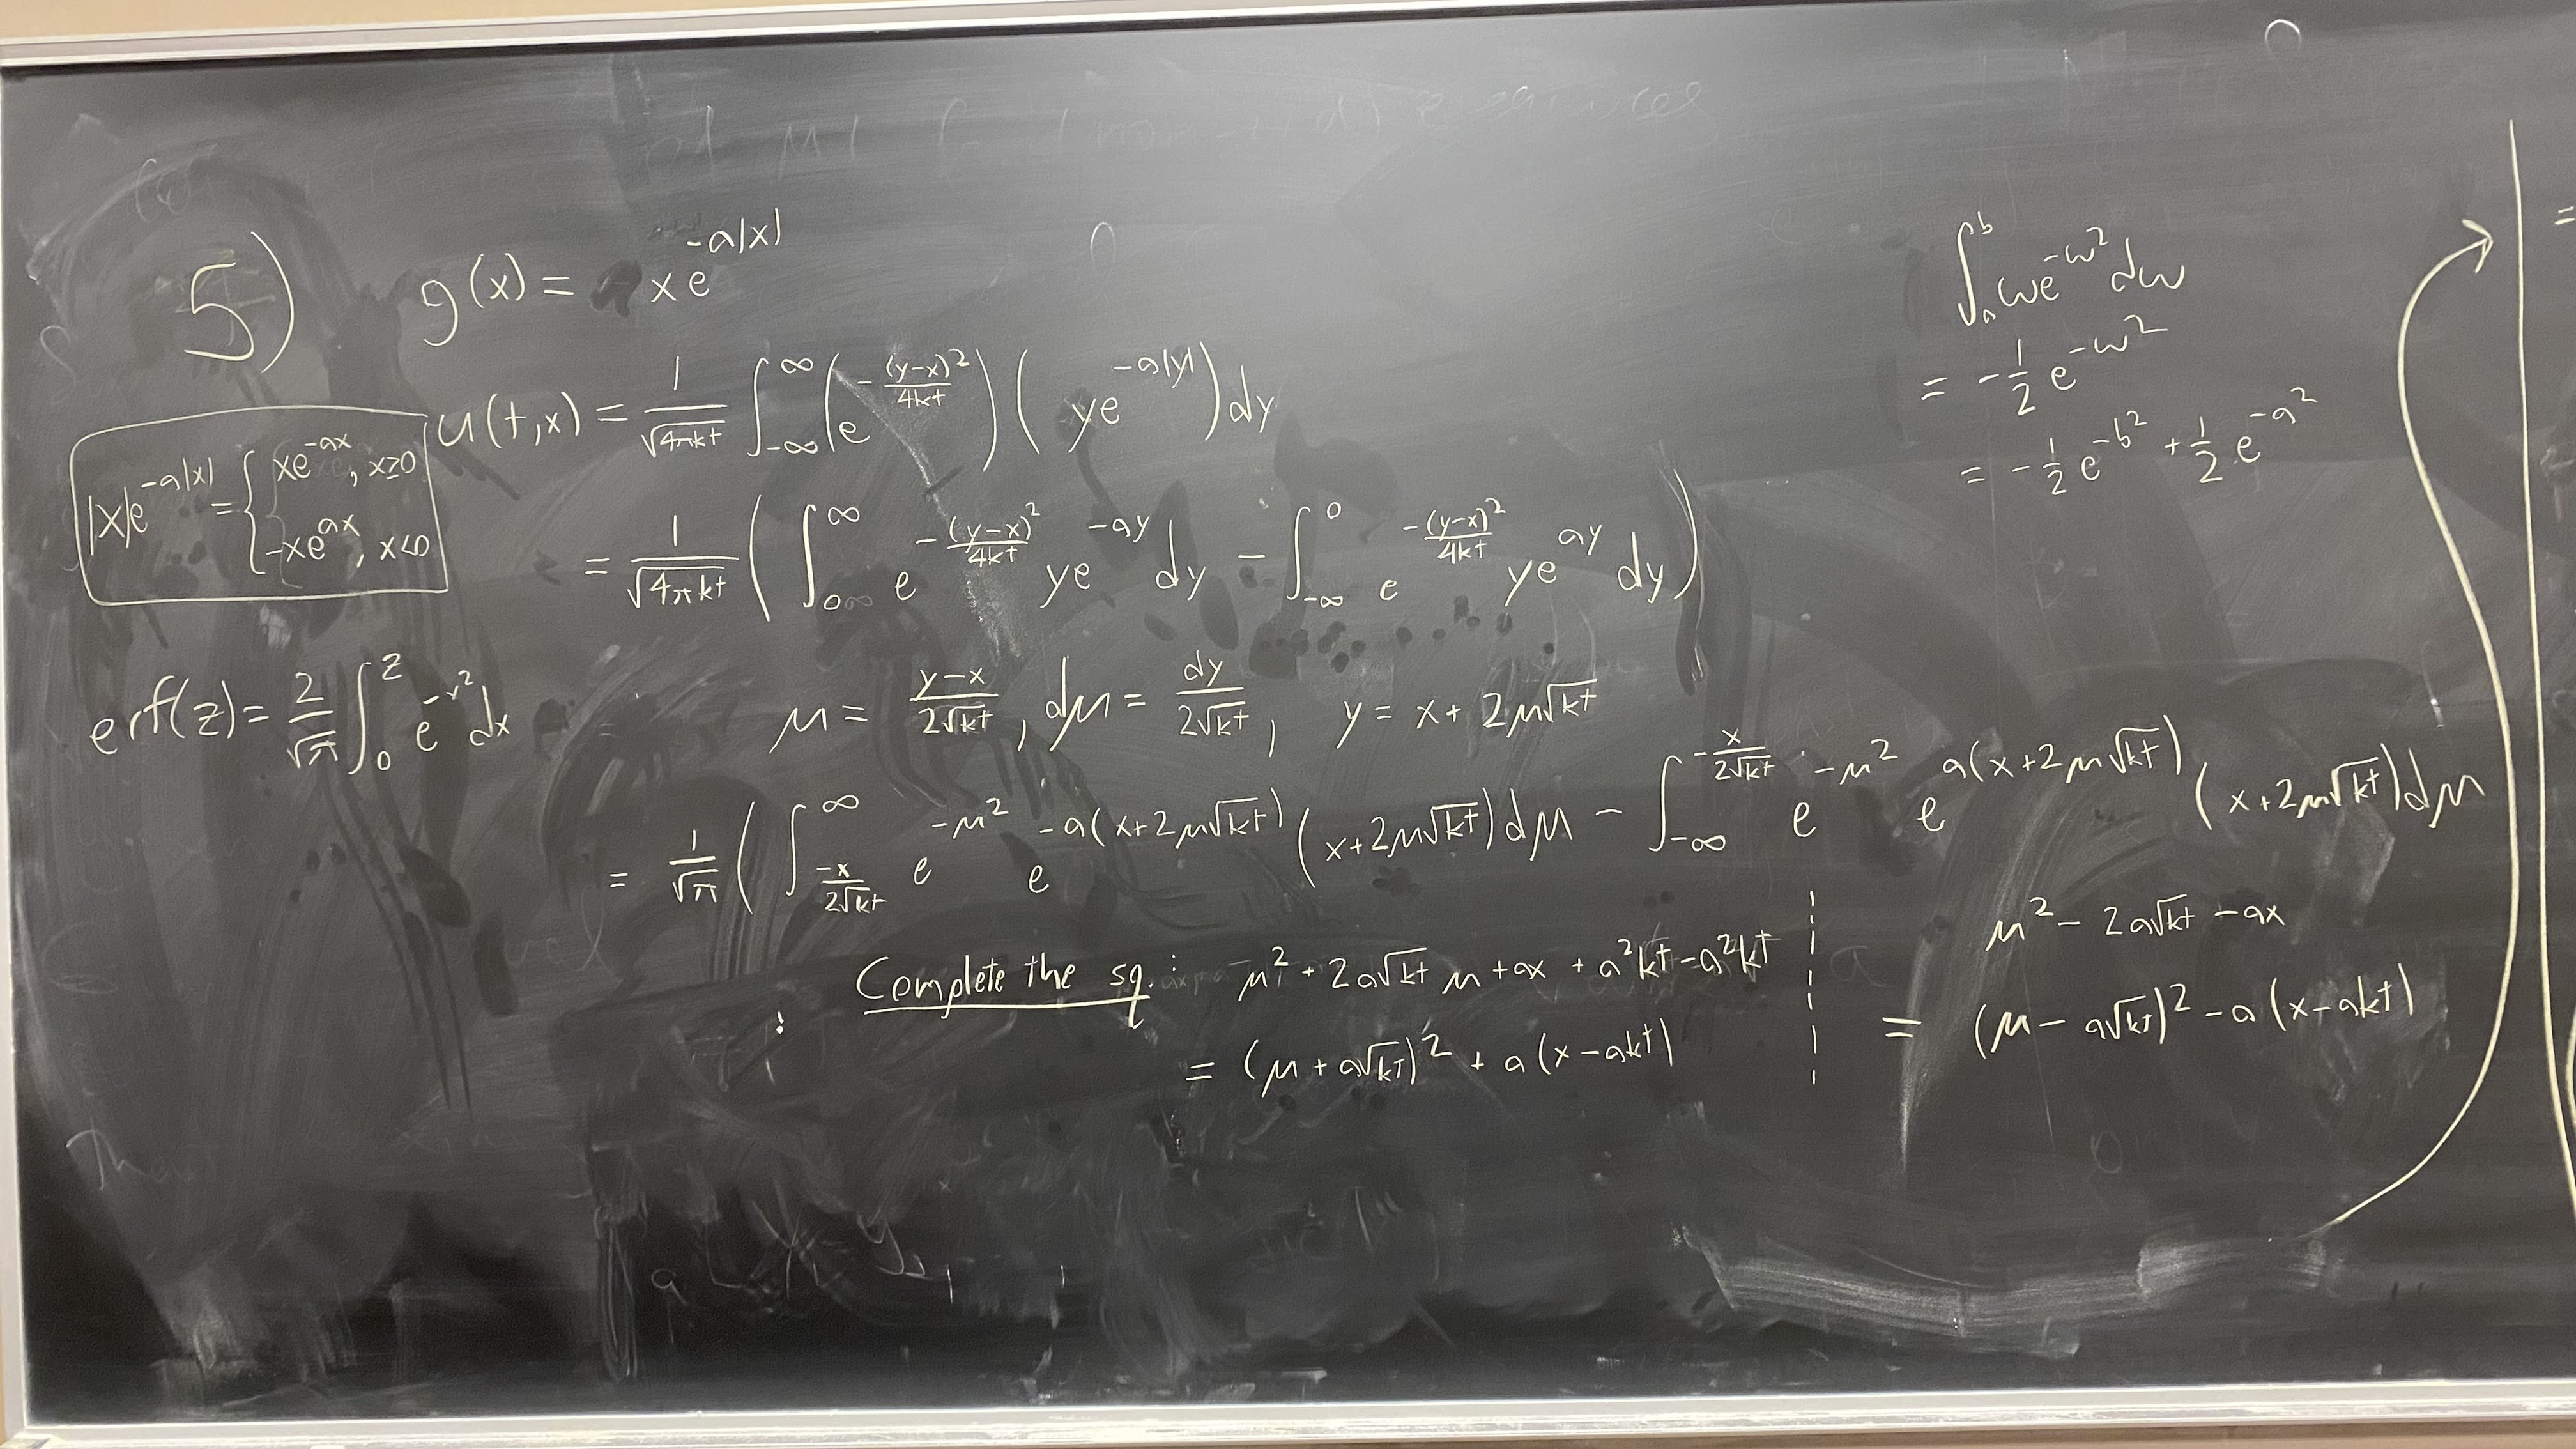
\includegraphics[width=\textwidth]{Problem 1.4-5.jpg}
    \end{figure}
    \begin{figure}[H]
        \centering
        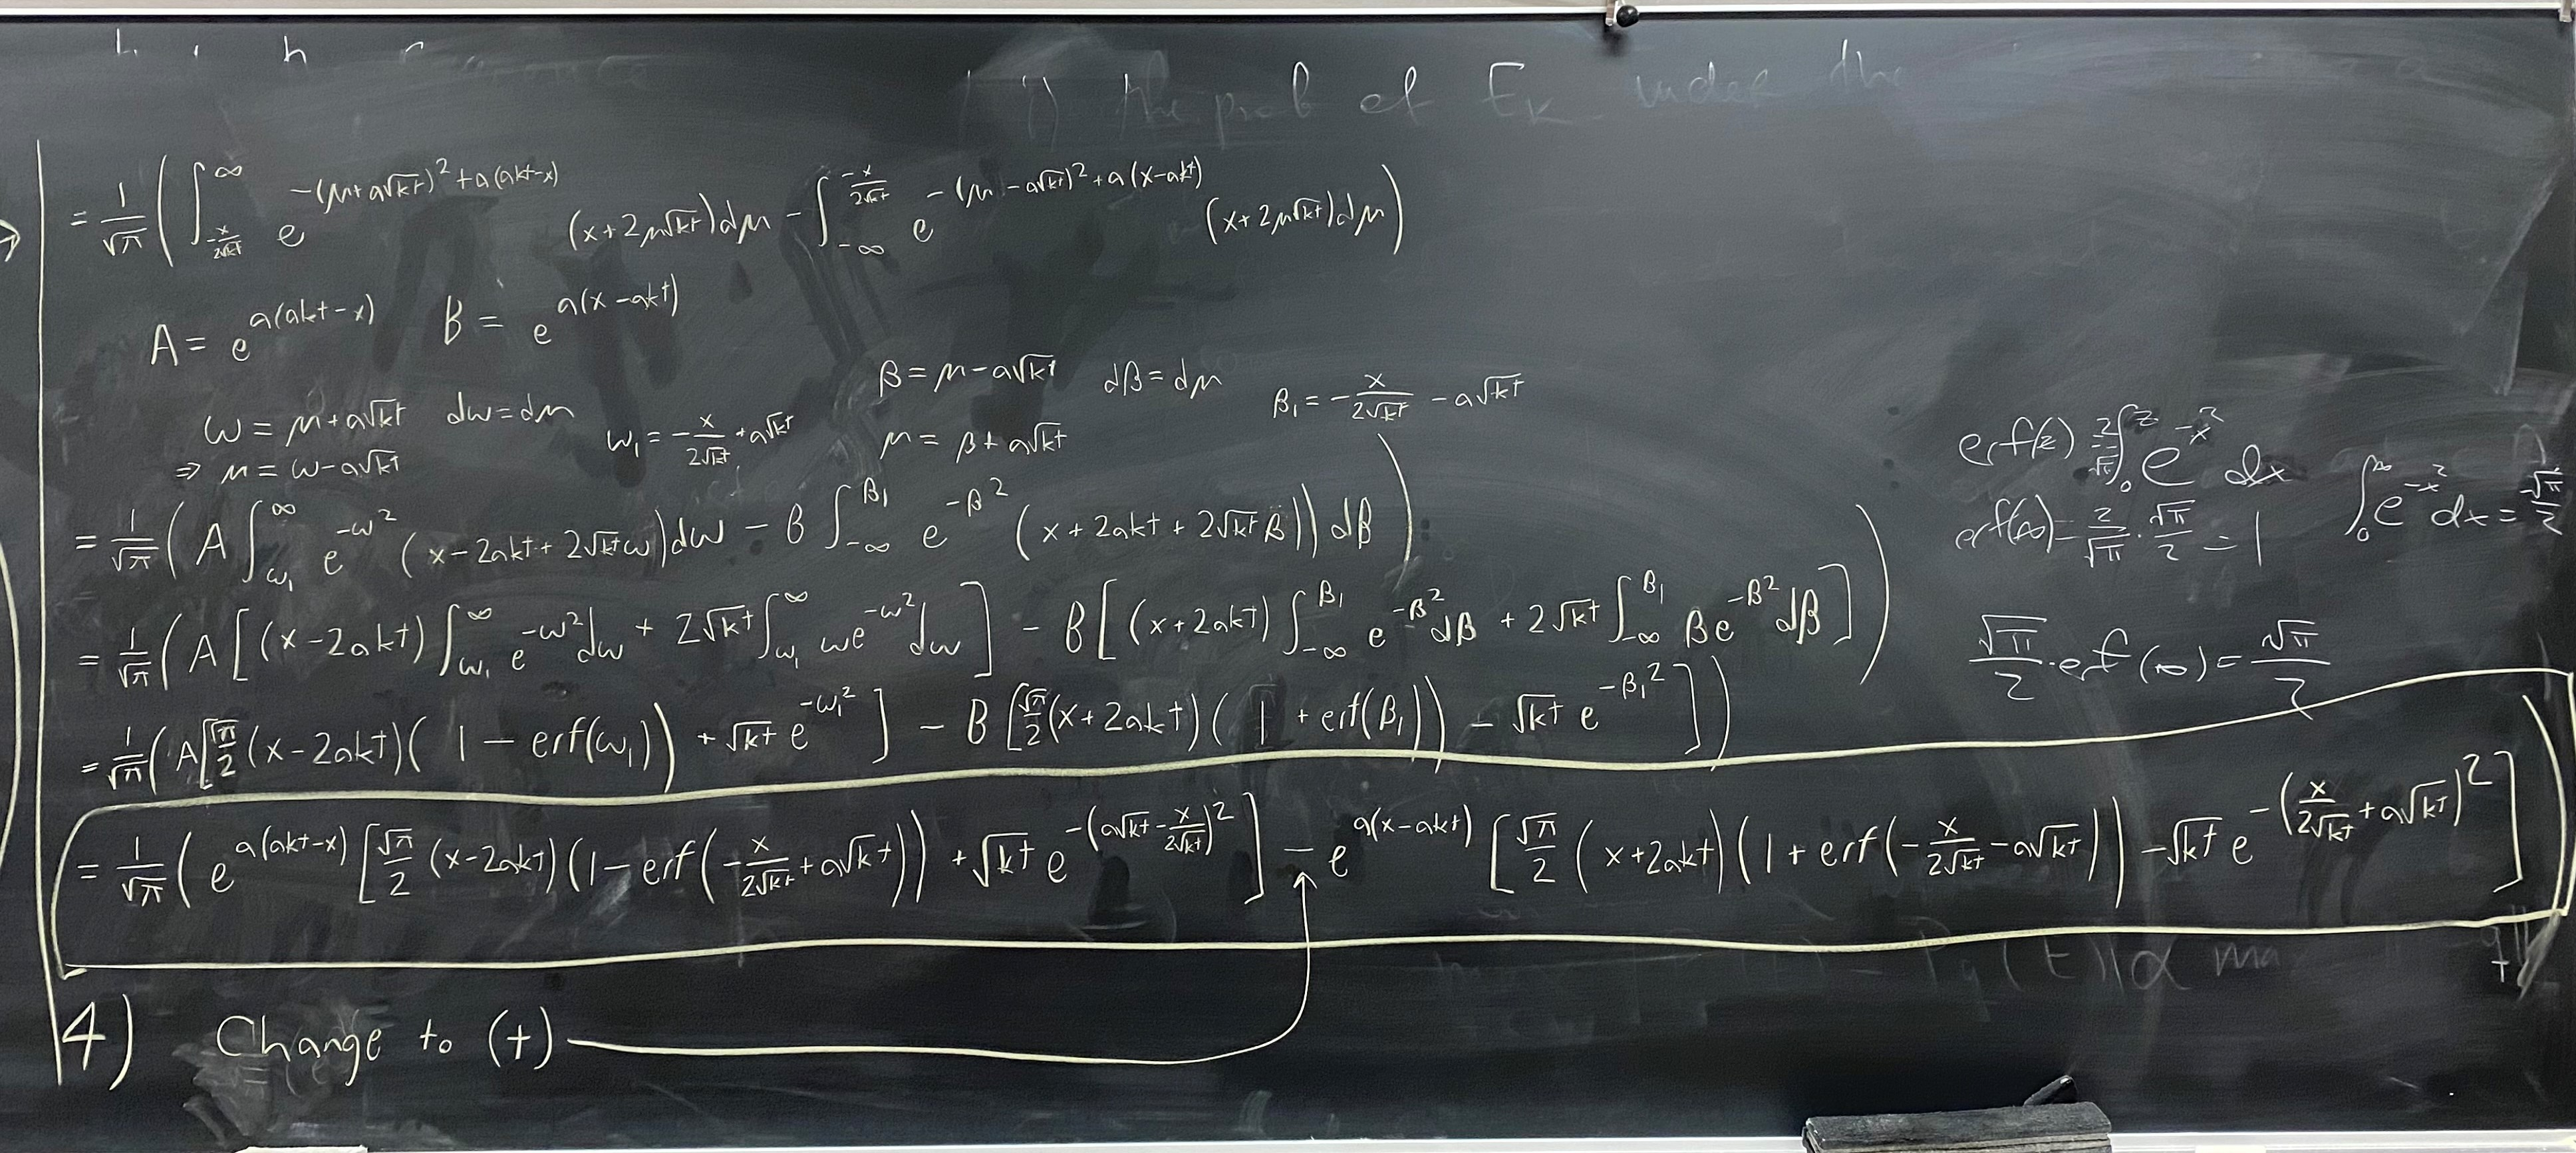
\includegraphics[width=\textwidth]{Problem 1.4-5 (2).jpg}
    \end{figure}
    \end{enumerate}
\end{ans}

\begin{boldenv}
    \underline{Problem 10}. \begin{enumerate}
        \item Consider the heat equation on $J = (-\infty, \infty)$ and prove that an energy
        \[ E(t) = \int_J u^2(x, t) dx \]
        does not increase; further, show that it really decreases unless $u(x,t) = const$;
        \item Consider the heat equation on $J = (0, l)$ with the Dirichlet or Neumann boundary conditions and prove that an $E(t)$ does not increase; further, show that it really decreases unless $u(x,t) = const$;
        \item Consider the heat equation on $J = (0, l)$ with the Robin boundary conditions \begin{align}
            u_x(0, t) - a_0u(0,t) &= 0\\
            u_x(L,t) + a_Lu(L,t) &= 0
        \end{align}
        If $a_0 > 0$ and $a_l > 0$, show that the endpoints to the decrease of $E(t) = \int_0^L u^2(x, t)\,dx$.\\
        This is interpreted to mean that part of the energy is lost at the boundary, so we call the boundary conditions radiating or dissipative.\\
        \textbf{Hint.} To prove decrease of $E(t)$, consider it derivative by $t$, replace $u_t$ by $ku_{xx}$ and integrate by parts.\\
        \textbf{Remark 1.} In the case of heat (or diffusion) equation an energy given by $E(t) = \int_J u^2(x, t) dx$ is rather mathematical artefact.
    \end{enumerate}
\end{boldenv}
\newpage
\begin{ans}
\begin{enumerate}
    \item \phantom{.}
    \begin{figure}[H]
        \centering
        \includegraphics[width = 0.45\textwidth]{Problem 10-1.jpeg}
        \includegraphics[width = 0.45\textwidth]{Problem 10-1 (2).jpeg}
    \end{figure}

    \item \phantom{.}
    \begin{figure}[H]
        \centering
        \includegraphics[width = 0.45\textwidth]{Problem 10-2.jpeg}
        \includegraphics[width = 0.45\textwidth]{Problem 10-2 (2).jpeg}
    \end{figure}
    \newpage
    \item \phantom{.}
    \begin{figure}[H]
        \centering
        \includegraphics[width = 0.45\textwidth]{Problem 10-3.jpeg}
        \includegraphics[width = 0.45\textwidth]{Problem 10-3 (2).jpeg}
    \end{figure}
\end{enumerate}
    
\end{ans}


\end{document}
